\chapter{Watts-Strogatz model}
\label{cha: Watts-Strogatz model}
The Watts-Strogatz model given the desired number of nodes, $N$, the mean degree $K$ and a parameter $0 \leq p \leq 1$ will construct an undirected graph without local clustering, in contrast with the Erdös-Rényi model in which there is local clustering.

To comprehensively analyze the influence of the parameter $p$ on both the clustering coefficient and the average shortest path, we will construct plots displaying the normalized progression of these metrics with varying $p$. Specifically, we will generate 100 random graphs of a specified size and mean degree, varying the parameter $p$ and taking the average. In Figure \ref{fig:ws}, the outcomes of this experiment are presented for a graph comprising 1000 nodes and an average degree of 2.

The depicted results confirm to the anticipated behavior of the random graph model. Initially, the average shortest path remains relatively stable until a specific $p$ value is reached, at which point it dramatically decreases to the normalized value of 0. This phenomenon indicates a highly interconnected network where almost all nodes are connected. Concurrently, the clustering coefficient starts off at a high value and then rapidly declines as the inter-connectivity intensifies, resulting in a large cluster and subsequently, a diminished coefficient.

\begin{figure}
    \centering
    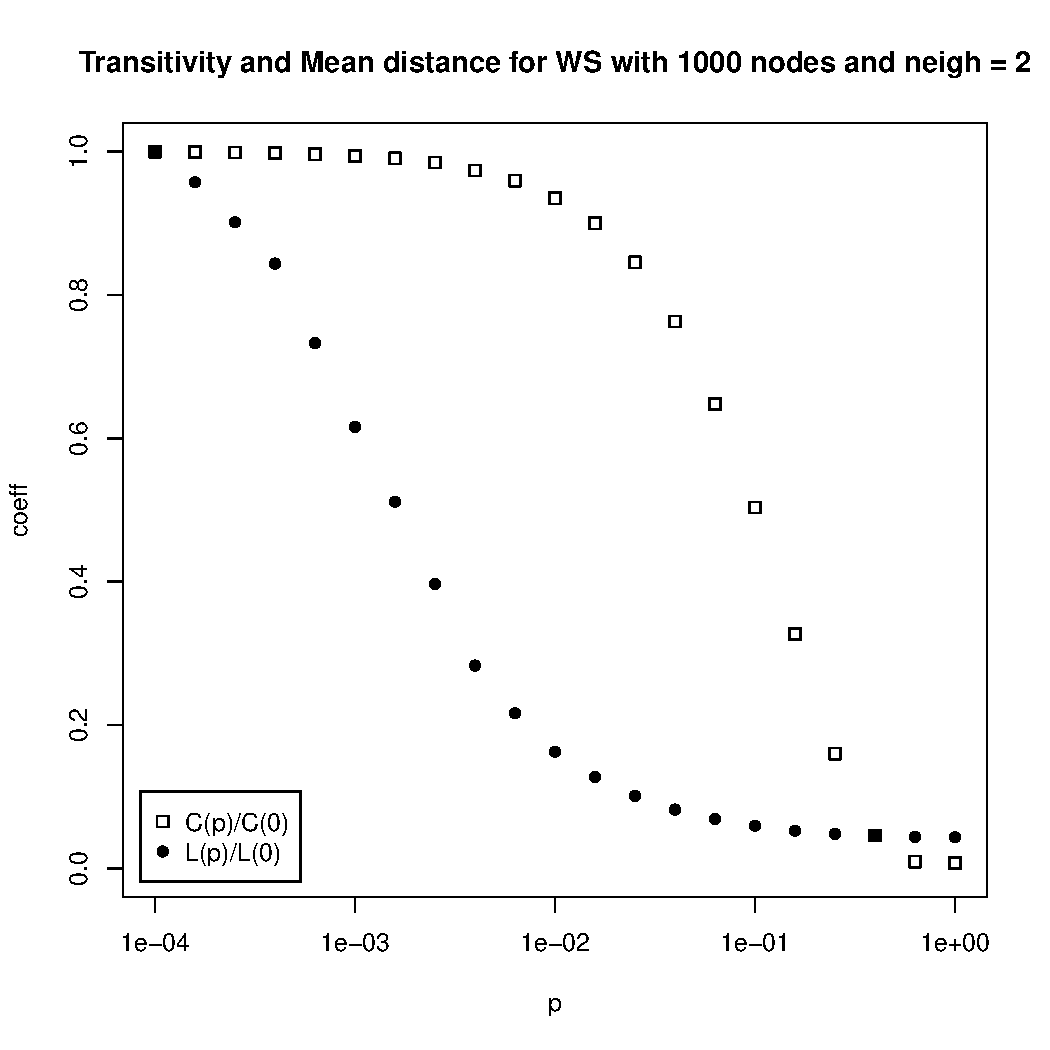
\includegraphics[width=0.66\textwidth]{figures/WS_neigh_2.pdf}
    \caption{Evolution of Clustering Coefficient $L(p)$ and the average shortest-path $C(p)$}
    \label{fig:ws}
\end{figure}

During our experimental investigations aimed at determining suitable mean degree values, an intriguing anomaly emerged, as depicted in Figure \ref{fig:ws_high_neigh}. Contrary to expectations, the Clustering Coefficient did not approach zero even at significantly high values of $p$. This behavior can be attributed to the inherent structure of the random graph model, where the presence of local clustering is preserved even at higher $p$ values. Additionally, our choice of normalization with respect to $L(0)$ contributes to this outcome, ensuring that the clustering coefficient doesn't deviate significantly from $L(0)$ due to the graph's elevated mean degree.

\begin{figure}
    \centering
    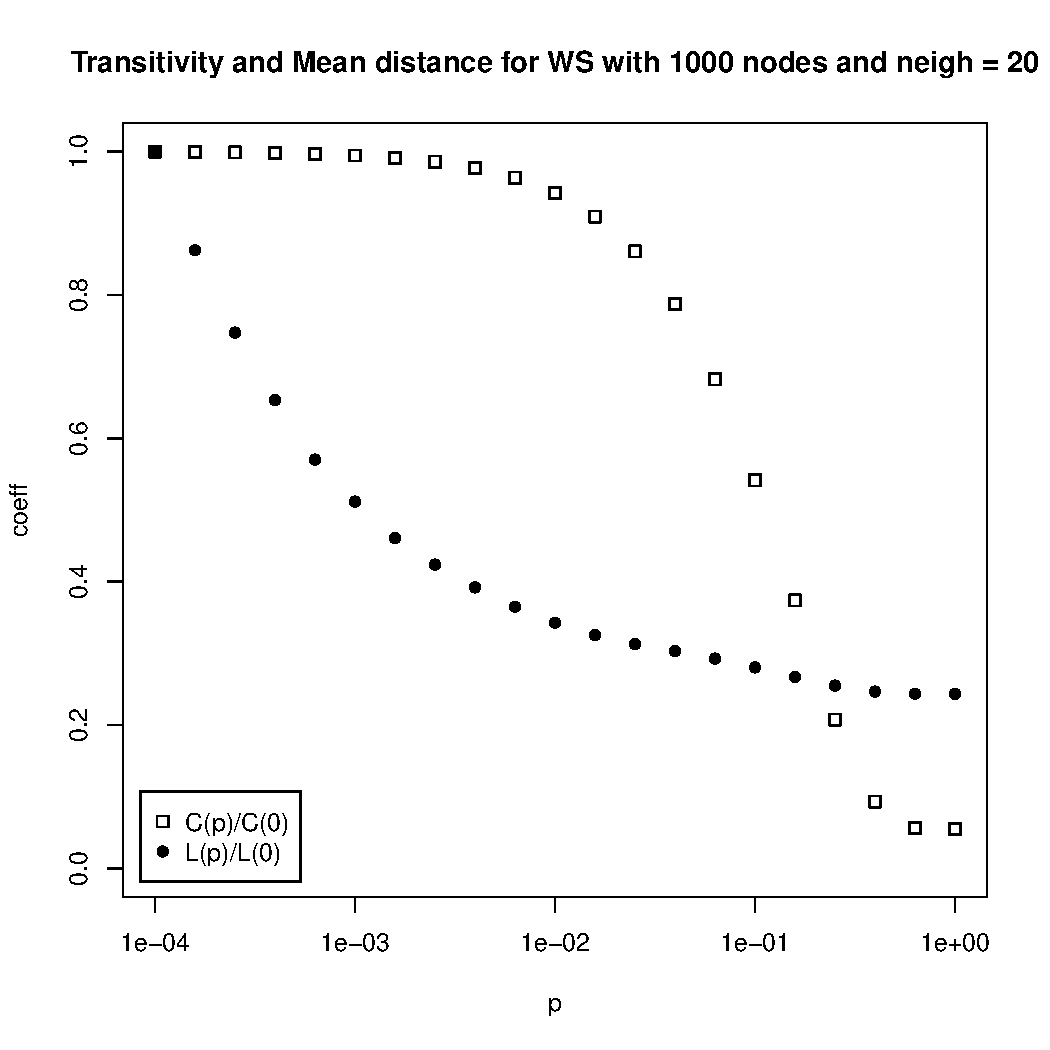
\includegraphics[width=0.66\textwidth]{figures/WS_neigh_20.pdf}
    \caption{Evolution of Clustering Coefficient $L(p)$ and the average shortest-path $C(p)$}
    \label{fig:ws_high_neigh}
\end{figure}